\documentclass{elsarticle}
\usepackage{amsmath}
\usepackage{amssymb,amsfonts,textcomp}
\usepackage{color}
\usepackage{array}
\usepackage{supertabular}
\usepackage{hhline}
\usepackage{hyperref}

\journal{Expert Systems with Applications}

\makeatletter
\newcommand\arraybslash{\let\\\@arraycr}
\makeatother

\begin{document}

\begin{frontmatter}

  \title{A Method for Enterprise Knowledge Management Process Modeling Based on
Business Process-Driven}

  \author[buaa]{Jun Wang\corref{cor1}}
  \ead{king.wang@buaa.edu.cn}

  \author[buaa]{Yunpeng Wu}
  \ead{yunpeng.wu@sem.buaa.edu.cn}

  \author[buaa]{Guannan Liu}
  \ead{lanleo.guan@gmail.com}

  \author[buaa]{Huili Wang}
  %\ead{wd33082208@126.com}

  \cortext[cor1]{Corresponding author}

  \address[buaa]{School of Economics and Management, Beihang University, \par
    Beijing 100191, P.R. China}
\begin{abstract}
Knowledge Management Process
(KMP) is the core issue of Knowledge Management (KM) in organizations.
It needs continuous improvement and is closely related with
corresponding Business Process (BP). Many knowledge management
practices in organizations, however, are less effective since
organizations failed to integrate KMP with BP. This study proposes a
methodology for knowledge management process modeling based on business
process-driven, providing better support for the collaboration between
BP and KMP and in turn continuously optimize knowledge management
process. This methodology includes the architecture of the business
process driven knowledge management process modeling system, the
depiction of business process, a knowledge management process modeling
methodology based on XML, the depiction and storage of the
driven-rules  extracting knowledge management process from  business process. Finally we give a case study of an aviation manufacturing
enterprise to illustrate how this methodology can support the
collaboration between its production design process and knowledge
management process. An implementation evaluation will also be
given to verify the methodology.
  \end{abstract}

  \begin{keyword}
    Knowledge management process; Business-driven; Process modeling;
    Driven rules
  \end{keyword}
\end{frontmatter}

\section{ Introduction}

\textrm{Among many organization assets,}\textrm{knowledge}\textrm{{ }}\textrm{is treated as a
critical driving force for attaining organization performance goals
because knowledge facilitates the better business decision makings in a
timely fashion\cite{han2009process}. There has been a growing interest in treating
knowledge as significant organizational resource\cite{alavi2001review}}.


The exploitation and management of
 knowledge  is becoming a new organization
model\cite{vandaie2008role}. Knowledge management characterizes a deliberate and
systematic approach to ensure the full utilization of the knowledge
base of an organization. Effective knowledge management is an
increasingly important source to achieve competitive advantage and a
key factor of the
success of modern organizations\cite{becerra2001organizational}, especially for production design
enterprises. Therefore knowledge management is receiving increasing
focus from scholars and organizers. Knowledge management process is an
important issue in knowledge management practice, which involves
knowledge creation, storage/retrieval, transfer and application.
Many knowledge management efforts
have been largely concerned with capturing, codifying,
storing and disseminating knowledge that is held by people in
organizations in the pursuit of strategic competitiveness. However,
since knowledge is created and utilized during the execution of
business processes, if knowledge is separated from the business process
context, it does not lead to the ability to take the right action for
target performance. Knowledge management is an evolving practice
\cite{davenport1998working}.\textrm{Desouza and
Awazu argued that the rare combination with organizations has limited
the use of Knowledge Management when considered in the context of
organizations\cite{desouza2003barriers,desouza2006four}. }


\textrm{In the course of knowledge utilization, Dalkir  stressed
the importance of a shared context: how to describe and organize
content so that intended end users are aware of its existence and can
easily access and apply this content\cite{dalkir2005knowledge}. Without appropriate contextual
information, }\textrm{knowledge can be isolated from other relevant
knowledge, consequently resulting in a limited or distorted
understanding\cite{ahn2005utilizing}.}


\textrm{As the notion of knowledge management matures, it is
increasingly clear that knowledge management is not just about
technology, and can not be realized simply as information systems.
}Knowledge management 
emphasize and expect collaboration between a wide spectrum of
contributors that range from people and processes to supportive
technologies in an organization. Business process is a collection of
interdependent activities or tasks organized to achieve specific
business goals. Business process provides the justification and
rationale for knowledge management process and can effectively drive
the optimization of it\cite{raghu2007business}. 
In order to survive in the current
competitive and global business environment, most organizations are
struggling to change their existing business processes into more agile,
product- and customer-oriented structures\cite{ballard2005business}. Similarly, organization
performance is achieved through the execution of business processes, so
business process and enterprise performance are closely
interrelated\cite{kang2007process}.


As business process becomes a core competency factor in
today's rapidly changing business environment, we need an
organization-level perspective on the relationships among
organization performance, business processes and knowledge in a
process-centered way. In order to maintain sustainability, it is
essential to establish a process-centered knowledge management model.
In an agile and flexible organization structure, process is a core
element of business operations. Business process utilizes
knowledge during the process execution. In turn, knowledge drives the process to improve
day-to-day operations. Then it is essential to establish a knowledge
model that categorizes the type of enterprise knowledge to be managed
and creates relationships between knowledge objects in a process driven
way.


In this paper, we proposes a business process driven methodology
for knowledge management process modeling, providing better support for
the collaboration between business process and knowledge management
process and in turn continuous optimizing knowledge management process.
This methodology includes the architecture of the business process
driven knowledge management process modeling system, the depiction of
business process, a knowledge management process modeling methodology
based on XML, the depiction and storage for the driven rules
extracting knowledge management process from
business  process and so on. Finally we
give a case study of an aviation manufacturing enterprise to illustrate
how this methodology can support the collaboration between its
production design process and knowledge management process, in which an
implementation evaluation will also be given to verify the
methodology.


\textrm{The rest of the paper is organized as follows. Section 2
identifies the }\textrm{{needs}}\textrm{ for better
business driven automation support for knowledge management process
modeling as well as briefly reviews the related works. Section 3
describes the architecture of the business process driven knowledge
management process modeling system. Section 4 represented the business
process models using UML. Section 5 depicts the knowledge management
process modeling methodology based on XML as well as its
implementation. The driven rules classification, inference principles
and the storage of driven-rules based on the
between
business process and knowledge management process are discussed in
Section 6. Section 7 depicts a
case study taking an aerial manufacturing  enterprise as the background. We
conclude the paper in Section 8 by summarizing our research
contributions }\textrm{and pointing out future research directions.}

\section{ Background and Literature Review}
\label{sec:backgr-liter-revi}

\subsection{Background}
\label{sec:background}


With the development of Knowledge Management (KM) theory, the
methods and techniques of KM that can be adopted are becoming more and
more. Many enterprises have already implemented KM to lift its
operation efficiency and competiveness, making themselves knowledge
enterprises. In the KM practice, a lot of enterprises have been aware
of the changes that KM brings to. For example,
employees' efficiency and customers'
degree of satisfaction have been improved, the cycle of products going
into market has been shortened and the market share greatly rises. KM
has penetrated in all the aspects of enterprise operation, bringing
about huge and sustaining revenue to the KM equipped enterprises.
However, some enterprises come across obstacles in implementing KM. The
main reasons are listed as follows,

\begin{enumerate}
\item  The planning and expectation for KM is inappropriate, or the
planning maybe too gigantic or the enterprise had not considered the
actual situation of itself when implementing its KM.
\item  There is a lack of correct cognition and professional
training inside the enterprises.
\item The support from the members in the organization is
insufficient. Some enterprises make KM their
employees' extra work, or they hopefully expect
employees would share their information and knowledge actively, or they
even force each department to devote a certain amount of knowledge and
so forth. On the other hand, they had not established a perfect KM
motivation mechanism; as a result employees may be averse to KM.
 \item Enterprise's organizational structure and
business process is incompatible with its KM. Knowledge management is not
only a technical problem, but also an adjustment of thinking patterns
and organizational structure. Currently enterprises are lack of
necessary reforms in their management and process, thus KM system had
not played its role to make itself a part in
enterprises' business activities.
\end{enumerate}



The obstacles in implementing KM come down to the disjointedness
between Knowledge Management Process (KMP) and actual business process.
KMP is a dynamic management process constructed by
enterprises' required knowledge set in their normal
operation, which is their core knowledge. The dynamicity of KMP resides
in the fact that the core knowledge set changes with
enterprises' growth and KMP changes with
enterprises' actual activities. The objective of the
dynamicity of KMP is to set up a perfect motivation pattern, and
finally result in high performance with continually optimizing process.
There are two significant characteristics of KMP: firstly, it is an
evolving process that can be improved continually; secondly, it is
closely related with organization's BP. One of the
most important factors for KMP's continual improvement
is that it must keep with the constant changes of BP; while the
business oriented character could also promote sustaining optimization
for BP.


Most researches on KMP focus on KM activities, which is vital
for understanding the essence of KM. Whereas there still exist some
problems:
\begin{enumerate}
\item Most KMP researches have paid little attention to actual KM
activities, disjointing with enterprises' BP, thus
some related research achievements cannot be put into practice.
Employees are required not only to undertake their own jobs but also to
be incorporate with KM projects, deeming that KM projects add
extra working burden to them. KM cannot realize its great value owing
to the disjointness with enterprises' BP.
\item   Existing KMP researches related with BP are usually limited
to conceptual level. Thus there is a critical need for new
methodologies and tools to facilitate efficient and effective
collaboration between BP and KMP and achieve business driven automation
as well.
\item  Many implementations have indicated that the compatibility
between KMP and BP will greatly affect the efficiency of KM.
\item The relationship between BP and KMP is rather complex, making
the maintenance of the relation an important task. Ideally when new
business requirements come into being, the Config-Mode should
completely or partly uses the knowledge of
coordination rule between BP and KMP to adjust KMP, but not
set out to design new KMP. To achieve the goal, enterprises have to
collect knowledge of driven- rules, and they should also consider
different roles and processes, such as related experts, business
process and KMP, etc\cite{yang2009product}.
\end{enumerate}


\subsection{Literature Review}
\label{sec:literature-review}



\textrm{There have been many ways to resolve the disjointness between BP
and KMP. Researchers and experts have done a lot in integrating KMP and
BP. }\textrm{Lai \& Fan, Nissan et al. suggested the importance of
}\textrm{{integrating}}\textrm{ KM and BPM (business
process management) towards PCKM (Process Centered Knowledge
Management) in order to maximize and optimize business
performance}\cite{lai2002workflow,nissen2000toward}. \textrm{{Besides }}\textrm{Kwan Hee Han, Jun Woo Park
(2009) proposed a concept of process-centered knowledge management
(PCKM) as well as a framework for}\textrm{{
}}\textrm{process-centered knowledge
model}\textrm{.}\textrm{\textcolor[rgb]{0.5019608,0.0,0.0}{
}}


\textrm{Therefore, interests in the notion of process-oriented knowledge
management (PKM) from academia and industry have been significantly
}\textrm{{increased}}\cite{jung2007integration}\textrm{.
There have been various efforts to introduce the process concept to
knowledge management (Knowledge Management) or the knowledge concept to
business process management (BPM) in order to combine the advantages of
the two
paradigms}\cite{berztiss2000knowledge,maurer98concept,maurer1999process,choi2004integrated}. In
the context of IPM, I. Choi, J. Jung and M. Song
proposed a comprehensive framework for
integrating Knowledge Management and
BPM\cite{choi2004integrated}.
\textrm{K.H. Han and }\textrm{{Maurer, F }}\textrm{et
al. proposed a MILOS system in order to integrate Knowledge Management
with project-planning and process
coordination}\cite{maurer2000merging}.
\textrm{Jung et al., J. Jung, I. Choi and M. Song further proposed an
}\textrm{{integration architecture}}for integrating knowledge
management systems  and business process management systems
 to combine the advantages of the two paradigms based on a
comprehensive framework that reflects lifecycle requirements of both
KM and BPM. The architecture, which is comprehensive
since it is derived from the extended requirements from the lifecycle
perspective, will provide a basis for research and development of
process-oriented knowledge management systems. A prototype system is
presented to demonstrate the feasibility of the proposed
architecture\cite{jung2007integration}.


\textrm{Jablonski, Horn, and Schlundt (2001) combined business process
modeling with Knowledge Management and developed process-oriented KMS
prototype for car
manufacturing}\cite{jablonski-process}.\textrm{{
}}\textrm{Woitsch and Karagiannis proposed a service-based
approach in which the KM services separate technical
implementation and conceptual requirements. However, the
}\textrm{relationship between KM services and
business process was not shown in their
study}\cite{woitsch2005process}.


\textrm{J. Leon Zhao has proposed a process-driven collaboration
methodology called }\textrm{\textit{COPLINK}}\textrm{ to better
facilitate knowledge intensive collaboration}\cite{zhao2006process}\textrm{. In addition, a pilot evaluation study about
}\textrm{\textit{COPLINK}}\textrm{ showed its positive impact in
practice}\textrm{. The advantage of
process-oriented knowledge management is that it can help users avoid
information overload and concentrate on important information which is
essential for company value
chains}\cite{millie2003knowledgescope}. \textrm{It can also improve the usability of knowledge in company and
the efficiency of implementing knowledge management
system}.\textrm{{
}}



\textrm{These researches provide integrating methods between BP and KMP
from different perspectives, which greatly promote sustaining
optimization of KM. However, it needs further research and practice on
KMP modeling.}
\section{ Context and the architecture of
BDKMS}
\label{sec:cont-arch-bdkms-1}
\textrm{The driven automation between BP and KMP can be realized by
information technology. We set this paper in a real KM project for the
product development department of an aviation manufacturing enterprise
in China, and then design a Business Driven KMP Modeling System
(}\textrm{\textit{BDKMS}}\textrm{). According to the general
architecture of expert systems\cite{dhaliwal1996use,
chau2002expert}, this paper presents the architecture of
}\textrm{\textit{BDKMS}}\textrm{, including three main parts namely
driver, user interface and knowledge acquisition facilities, as is
shown in Fig.1.}


  \begin{figure}[ht]
    \centering
    \scalebox{0.75}{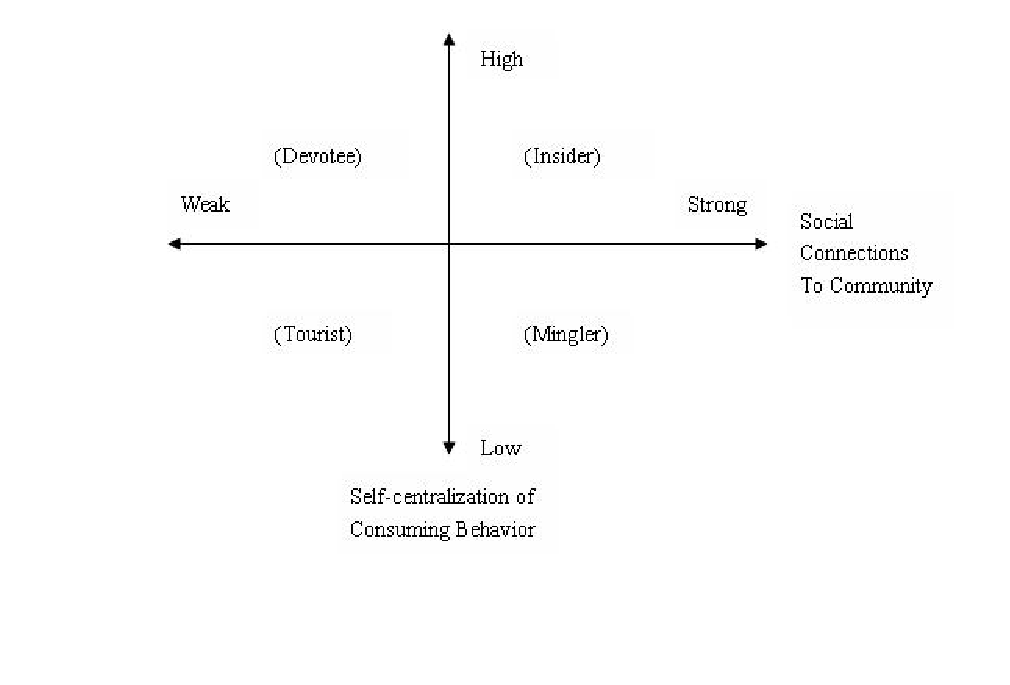
\includegraphics{01}}
    \caption{ The architecture of BDKMS}
  \end{figure}


  \begin{enumerate}
  \item Driver: Driver is the core component of the working
system\cite{curtis2005business}. Through collaboration of diver-rules base, global database,
interpreter and inference engine, the driver of
BDKMS constructed.
  \begin{enumerate}
\item 
\textrm{Driven-rules Base: As the core component of
}\textrm{\textit{Driver}}\textrm{, Driven-rules stores expert knowledge
in different knowledge representation form such as Semantic Web,
FrameNet and Predicate Logic. The most commonly used is Production
Rules in the form of "If...Then..." to
represent knowledge\cite{huang2009designing}. In this paper, Driven-rules stores and manages the
driven-rules between BP and }\textrm{KMP, and they are also represented
in Production Rules.}
\item 
\textrm{Global database : Global database stores current BP models, new
BP models inputted by users and current KMP models, etc. Inference
engine would use the knowledge in the knowledge base and the facts in
the global database to model new KMP.}
\item 
\textrm{Inference Engine: Inference Engine is a set of operation rules
involving the decomposition and evolvement of driven-rules, which is
independent of specific expert system and thereby can be applied to
similar systems.}
\item 
\textrm{Explanatory: It is used to explain the outputted new KMP models,
from which users can understand the process that the change of 
specific BP drives the change of the KMP.}
\end{enumerate}
\item User Interface: It is the
aggregate means by which users interact with the system, including
input of new BP models, output of new KMP models, and maintenance of
Driven-rules Base and so on.
\item Knowledge Acquisition Facility: It is used
s to facilitate the maintenance of the Driven-rules Base. The
principle is that it transfer the driven-rules from
Chinese form to coded form on the
basis of some preestablished strategies, and then store them in the
knowledge base.
  \end{enumerate}



\textrm{The working process of }\textrm{\textit{BDKMS}}\textrm{ is as
follows: users firstly input a new BP model through the
}\textrm{\textit{User Interface}}\textrm{, and then the system will
compare it with the existing BP models stored in the Global Database
and result in a series of changed parameters, triggering the Inference
engine. The Inference Engine would firstly store the changed parameters
in the Global Database, search the matched rules in the Driven-rules
Base, and then make inference through corresponding reasoning logic to
form a Meta-Rules set that can be executed directly by the system.
Furthermore, these rules can change the KMP model and set up a new KMP
model explained through Explanatory. The Inference Engine could drive
the change of KMP modeling, and finally the system would output the
new KMP model through the }\textrm{\textit{User Interface}}\textrm{ in
the form of graph, document, etc.}


\textrm{Existing driven-rules are based on the requirement of current BP
and KM of enterprise. With the extensive application and the
continual development of the enterprise, existing rules cannot fully
meet the need of new BP and KM. Experts analyze the relationship
between new BP and KMP, and then input the driven-rules between them
into the system through the interface. }\textrm{\textit{Knowledge
Acquisition Facilities}}\textrm{ code these rules and store them in the
Driven-rule Base, so that the knowledge base is maintained and upgraded
constantly to meet the development of the enterprise.}

\section{ Business Process
Depiction}
\label{sec:busin-proc-depict-1}

\textrm{BP is crucial for enterprises' operation and
management, so efficient implementation of BP is one of the key factors
to ensure enterprises' success. Besides, BP is a structure to depict
the related activities and their interactions. It is used to
manufacture products and create services, and finally achieve
enterprises' established goal, thus
enterprises' BP has an enormous influence on their
global achievements\cite{hammer2003reengineering,kueng1997goal}.}


\textrm{Simultaneously, enterprises' BP is also the
place to use and create knowledge, closely related to KM. Generally
speaking, roles, states and activities are the main factors in BP. BP
modeling is an effective tool to manage enterprises'
BP change\cite{chung2003knowledge}. There are many BP modeling methods, among which Unified
Modeling Language (UML), Business Process Modeling Notation (BPMN),
Entity-relationship modeling, BPR flow graph, state-driven modeling
language are common. Compared with other modeling methods, UML
eliminates the needless differences in notation and terminology;
moreover, its expressivity is articulate and unanimous.  This research
adopts UML to model BP.}


\textrm{BP modeling may vary with the organizational structure. Some
enterprises are in a linear structure, some are in functional
structure, or some others are mixed. The product development department
of the aviation manufacturing enterprise in China mentioned above is
just in a tree organizational structure, in which the top layer is the
design institute, the second are departments and the bottom are teams and
groups. There are several departments in the design institute, and each
one owns several teams and groups. Usually we use state diagram,
activity diagram and use case diagram in UML to comprehensively
describe the BP modeling for the design institute from different
perspectives, based on the three main elements of
enterprise's BP. Engineering design is a
knowledge-intensive process, including conceptual design, detailed
design, engineering analysis, process planning, process design and
outcome evaluation, in which each section touches on knowledge and
experiences in all areas\cite{chen2005developing}.}


\textrm{State diagram is used to track the states of each business
resource as well as the incidents resulting in states changing. The BP
in every  departments
enterprise can be classified into 4 categories: Design Proposal
Submission Process;}
\textrm{Proposal Modification Process; Proposal Archiving Process and
Proposal Downloading Process. Besides, examining and censoring are
included partially or wholly in each process. In order to facilitate
the indication, we take the Design Proposal Submission Process as an
example with its corresponding State Diagram illustrated in Fig.2.}

  \begin{figure}[ht]
    \centering
    \scalebox{0.75}{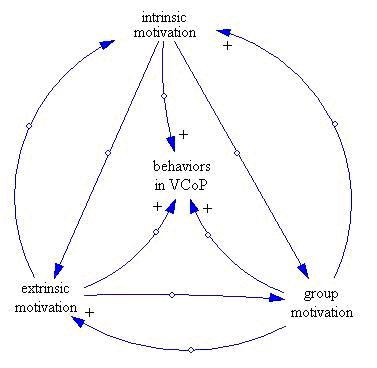
\includegraphics{02}}
    \caption{ State diagram of the design proposal submission process}
  \end{figure}


\textrm{Activity Diagram demonstrates a series of sequential activities,
which is one of the most important tools to represent BP in UML. The
Activity Diagram of the BP mentioned above can be inferred from Fig. 2,
so the related details will not be repeated here.}


\textrm{Use Case Diagram describes the business contents from the
perspective of users, so it is able to effectively extract various
roles and their functions in BP. The principal roles of the designing
department are institute members, team members, team leaders,
department members and directors, institute leaders, chief architect,
and so on. There are inheritances among these roles: all }\textrm{roles
inherit institute members, team leaders inherit team members,
department directors inherit department members, directors and chief
architect inherit institute leaders. All the use cases can be divided
into three groups: institute members Use Case, team leaders Use Cases
and department director Use Case. Generally, institute member is in
charge of proposal designing, submission and modification, while team
leader is responsible for censoring and directors for auditing.}

\section{ Knowledge management Process Modeling
Methodology}
\label{sec:knowl-manag-proc-1}

\textrm{Knowledge representation converts acquired knowledge to the
format that can be identified by the Knowledge Based System (KBS)\cite{berggren1998knowledge}. The
objective of KMP modeling is to generate knowledge process
representation documents, among which XML is often used
\cite{jovanovic2005achieving}. Knowledge
Management System (KMS) can reflect the change of KMP by these XML
documents. There are a number of mature process modeling methods, but
most of them are BP oriented. This paper adopts XML modeling to model the KMP, and finally
form XML documents representing knowledge process.}

\subsection{ XML modeling methodology}
\label{sec:xml-model-meth}




\textrm{The main body of XML is made up with XML tags and elements. XML
tag is defined as start tag, end tag and all the content between them,
including attribute, notation, text and sub-element. The content of tag
contains element name and all the attributes. A formalized
representation method based on the XML structure is adopted in this
paper, as is shown in Fig.3.}

  \begin{figure}[ht]
    \centering
    \scalebox{0.75}{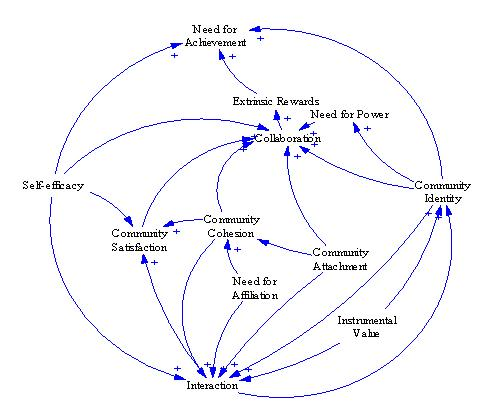
\includegraphics{03}}
    \caption{ XML modeling methodology}
  \end{figure}


\subsection{A knowledge management modeling case}


As for KMP, the main body is the knowledge base. The knowledge
base is usually composed of Uniform Resource Identifier, Level, Title,
Common Property and Special Property, which can be represented by a
multi-tuple: $KB(URI, L, T, CP, SP_1, SP_2,\ldots,SP_n)$.


We take the process of adding a knowledge base as an example to
illustrate the KMP modeling process. Usually adding a knowledge base requires three
procedures:
\begin{enumerate}
\item Identify the knowledge base level L;
\item Identify other required parameters;  




According to $KB(URI, L, T, CP, SP_1, SP
_2,\ldots,
SP_n)$ , other required parameters are: (1)URI, for a
first level knowledge base, the URI can be defined as
$URI=urn:kbs:material/**$,
in which confliction with existing URI should be avoided when defining
“**” by ourselves; while for a second level knowledge base, its URI
should be in the form of
\textrm{\textit{“urn:kbs:material/zgpx/**”}}\textrm{, the rule in
defining “**” is similar to that in the first level and
}\textrm{\textit{“urn:kbs:material/zgpx/”}}\textrm{ represents the
first level knowledge base it belongs to. Similarly, if there is the
third level, its URI should be like
}\textrm{\textit{“urn:kbs:material/zgpx/jcpx/**”}}.
(2)Level(L): Level can be obtained from the previous
procedure.
(3)Title(T): Title can be defined according to the
requirements.
(4)Common Property(CP): All the common properties are
defined by the system, which can be added in module. Any single
knowledge base cannot modify common property independently.
(5)Special Property(SP): We can define the special property
name and quantity freely for a specific knowledge base.

\item  Add the knowledge base

\end{enumerate}
\textrm{Based on the  procedures, adding
knowledge base involves adjustment on three modules: URI
definition, upfront demonstration and property definition.
}\textrm{{According to the parameters L and
URI,}}\textrm{ the URI definition module can be modeled as Fig.4.}

  \begin{figure}[ht]
    \centering
    \scalebox{0.75}{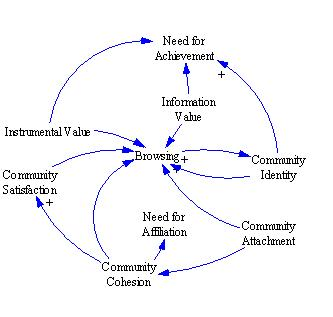
\includegraphics{04}}
    \caption{ The URI definition module}
  \end{figure}


\textrm{The XML document segment generated by the model illustrated in
Fig. 4 is as follows:}

{\itshape
{\textless}kid:id
rdf:about="urn:kbs:material/zgpx"{\textgreater}}

{\itshape
{\textless}kid:is
rdf:resource="urn:kbs:material"
/{\textgreater}}

{\itshape
{\textless}kid:generator
kid:pattern="\$node\$/material/zgpx/\$sequence\$"
/{\textgreater}}

{\itshape
{\textless}/kid:id{\textgreater}}


\textrm{Required parameters for upfront demonstration are
}\textrm{\textit{L}}\textrm{, }\textrm{\textit{URI}}\textrm{ and
}\textrm{\textit{T}}\textrm{, and the module of property adding calls
for the parameters of}\textrm{\textit{ L}}\textrm{,
}\textrm{\textit{URI}}\textrm{, }\textrm{\textit{CP}}\textrm{ and
}$SP_i$\textrm{. Both models can be constructed
according to the elements graph and the related details in Fig.3, so
that it will not be repeated here.}

\section{The depiction and storage of driven
rules}
\label{sec:depict-stor-driv-1}

\textrm{Driven-rules can realize business driven only by formalized
representation methods. Knowledge representation plays an important
role in knowledge inference. Knowledge representation methods are
various, including Predicate Logic, Production Rule, Semantic Web,
Script, Petri Net, Object }\textrm{Oriented method and so on, among
which Production Rule has been widely applied because of its
understandability and simplicity\cite{wen2008mobile}. The general form of Production Rule
is: IF A Then B. Andrzej Macioł has modeled business rule by the
methodology of Production Rule, and these rules are stored in the
relational database in his paper. Furthermore, a case is provided in
his paper to prove the validity of this method\cite{maciol2008application}. Therefore in this
paper, the Production Rule methodology is also adopted to depict the
driving relationship between BP and KMP.}

\subsection{ Driven-rules and their inference logic/ principle}
\label{sec:driven-rules-their-1}
Driven-rules are composed of rule ID, rule precondition and conclusion,
called Rule Element. Their formal expression is as follows:


\textrm{Rule ID: }(1)\textrm{\textit{DR [i]}}\textrm{; (2) Rule
Precondition: }\textrm{\textit{RP}}\textrm{
{\textless}}\textrm{\textit{ij}}\textrm{{\textgreater},
where}\textrm{\textit{ i}}\textrm{ equals the Rule ID
and}\textrm{\textit{ j }}\textrm{starts from 1;}
(3) Rule Conclusion: \textrm{\textit{RC}}\textrm{
{\textless}}\textrm{\textit{ik}}\textrm{{\textgreater}, where
}\textrm{\textit{i}}\textrm{ represents Rule ID and }\textrm{\textit{k
}}\textrm{starts from 1; (4)The relations between preconditions.
And: expressed with the symbol ${\cap}$, means that all the
preconditions should be satisfied; Or: expressed with the symbol
${\cup}$, means that one or more preconditions be satisfied; And/or:
expressed with the symbol ${\odot}$, means only one can be satisfied;}


\textrm{In order to infer the rules, the definition of Meta-Rule is
illustrated in Definition 1 as follows:}


\textrm{Definition1: Meta-Rule is the most fundamental rule that cannot
be decomposed but can be directly executed by the expert system. Rules
in realities must be decomposed into Meta-Rules because they are
usually complicated. This paper classifies the complicated rules into
four categories: }\textrm{\textit{SS}}\textrm{,
}\textrm{\textit{MS}}\textrm{, }\textrm{\textit{SM}}\textrm{,
}\textrm{\textit{MM}}\textrm{, besides, it also depicts the procedures
of decomposing the complicated rules into Meta-Rules.}

{
(1)Single-Precondition Single-Conclusion Rule(SS)}


\textrm{Rule in the form of }\textrm{\textit{DR[i] =If
RP{\textless}x{\textgreater} Then
RC{\textless}y{\textgreater}}}\textrm{ is called Single-Precondition
Single-Conclusion Rule. They can be directly executed by the expert
system. Such rules and the MAS rules described later can be considered
as Meta-Rule uniformly. Therefore all the complicated rules in this
paper can be decomposed into the two types of rules.}

{
(2) Multi-Preconditions Single-Conclusion Rule(MS)}


\textrm{MS can be divided into two categories according to the relations
of the preconditions.}
a) Multi-And-Preconditions Single-Conclusion Rule(MAS): Rule
in the form of \textrm{\textit{DR[i] =If
RP{\textless}i1{\textgreater}…${\cap}$RP{\textless}in{\textgreater}
Then RC{\textless}y{\textgreater}}}\textrm{ is called MAS rule. Only
when all the preconditions are true, the conclusion is true. Therefore,
MAS rule is another kind of Meta-Rule and cannot be decomposed.}
b) \textrm{Multi-Or-Preconditions Single-Conclusion Rule(MOS): Rule in the
form of }\textrm{\textit{DR}}\textrm{[}\textrm{\textit{i}}\textrm{]=If
}\textrm{\textit{RP}}\textrm{{\textless}}\textrm{\textit{i1}}\textrm{{\textgreater}…${\cup}$}\textrm{\textit{RP}}\textrm{{\textless}}\textrm{\textit{in}}\textrm{{\textgreater}
Then}\textrm{\textit{
RC}}\textrm{{\textless}}\textrm{\textit{y}}\textrm{{\textgreater} is
called MOS rule. MOS rule can be decomposed into several SS rules,
i.e.:}


$DR[i_1]=If \ RP<i_1> \ Then \  RC<y>$

$\cdots\cdots$

$DR[i_n]=If \ RP<i_n> \ Then \  RC<y>$

\textrm{These sub rules
must be executed in traversal until
}\textrm{\textit{RC}}\textrm{{\textless}}\textrm{\textit{y}}\textrm{{\textgreater}
or the last sub rule is executed.}


(3) Single-Precondition Multi-Conclusions Rule (SM)


\textrm{According to the relationship between the conclusions, SM rule
is divided into two sub categories:}
a) Single Precondition Multi-And-Conclusion Rule(SMA): Rule
in the form of $DR[i] =If \  RP<x> Then \  RC<i_1>\ldots \cap RC<i_n>$
is called MAS rule. The SMA rule can be decomposed into several SS
rules, i.e.


\textrm{\textit{DR[i1]=If \ RP{\textless}x{\textgreater}Then
RC{\textless}i1{\textgreater}……DR[in]=If
\ RP{\textless}x{\textgreater}Then
RC{\textless}in{\textgreater}}}\textrm{, where the relationship between
these sub rules }\textrm{\textit{DR[i1],…,DR[in]}}\textrm{ is and; thus
all of them must be executed.}



b) Single Precondition Multi-Or-Conclusions Rule (SMO)
Rule in the form of $DR[i]=If \
RP<x>\ Then \
RC<i_1> \ldots\cup RC<i_n>$\textrm{
is called SMO rule and it can be decomposed into several SS rules,
i.e.}


$DR[i_1]=If \ RP<x> \ Then \
RC<i_1>\ldots DR[i_n]= If
\ RP<x>\ Then \
RC<i_n>$\textrm{, where the relationship between
these sub rules
}$DR[i_1],\ldots,DR[i_n]$
is Or. Therefore, any one or more than one of them would be executed.

{
(4) Multi-Preconditions Multi-Conclusions Rule (MM)}


\textrm{According to the relationship between the preconditions and the
relationship between the conclusions, we divide MM rule into four sub
categories:}


a) Multi-And-Preconditions Multi-And-Conclusions Rule (MAMA).


\textrm{The MAMA rule can be decomposed into several MAS rules and all
the sub rules have to be executed in the way that is similar to the SMA
rule.}


b) Multi-And-Preconditions Multi-Or-Conclusions Rule(MAMO).


\textrm{The MAMO rule can be decomposed into several MAS rules and any
one or more than one of them should be executed, similar to the SMO
rule.}

c) Multi-Or-Preconditions Multi-And-Conclusions Rule(MOMA)


\textrm{The MOMA rule can be decomposed into
}$n*n$\textrm{ SM rule and these rules can be divided
into }\textrm{\textit{n}}\textrm{ groups according to the preconditions
and the conclusions. The executing principle is similar to the MOS rule
within each group, while it is similar to the SMA rule between
groups.}


d) Multi-Or-Preconditions Multi-Or-Conclusions Rule (MOMO).


\textrm{The MOMO rule can be decomposed into
}$n*n$\textrm{ SS rule and these rules can be divided
into}\textrm{\textit{ n}}\textrm{ groups}


\textrm{according to the preconditions and the conclusions. The
executing principle is similar to the MOS rule within each group, while
it is similar to the SMO rule between groups.}


\textrm{Based on the BP and KMP of the aviation manufacturing
enterprise, this paper uses several normal changes in its BP as driven
factors to depict the main driven-rules.}


\subsubsection{ Business contents change}
\label{sec:busin-cont-change}




\textrm{Business change mainly influence the change of the knowledge
base, for example, business
adding(}\textrm{\textit{B}}\textrm{\textit{\textsuperscript{+}}}\textrm{)}\textrm{\textit{
}}\textrm{results in knowledge base adding, business
deleting(}\textrm{\textit{B}}\textrm{\textit{\textsuperscript{{}-}}}\textrm{)}\textrm{\textit{
}}\textrm{results in knowledge base deleting and business modifying
(}\textrm{\textit{B\^{}}}\textrm{)}\textrm{\textit{ }}\textrm{results
in knowledge base modifying. As discussed in 5.2, a knowledge base in
an enterprise can be formally depicted as}
$KB(URI, L, T, CP, SP_1, SP_2,\ldots,SP_n$). The influence of business contents change on KMP can
be displayed in Table 1 by the driven-rules,


\begin{table}[!htb]
\scriptsize{}
\tablehead{}
\tablecaption{Driven-rules related to business contents
change}
\begin{supertabular}{m{0.97885984in}|m{2.1636598in}|m{2.49486in}}
\hline

\centering \bfseries Driven-factors &
\centering \bfseries Driven-rules and
decomposition &
\centering\arraybslash \bfseries Remark on
expressivity\\\hline
\centering \sffamily
\textrm{\textbf{\textit{B}}}\textrm{\textbf{\textit{\textsuperscript{+}}}}
&
\sffamily \textrm{\textbf{\textit{DR[1]=IF
B}}}\textrm{\textbf{\textit{\textsuperscript{+}}}}\textrm{\textbf{\textit{
THEN KBA}}} &
\bfseries\itshape KBA=KBA(KB\{URI, L, T, CP,
SP1, …SPn\})\\\hline
\centering \sffamily
\textrm{\textbf{\textit{B}}}\textrm{\textbf{\textit{\textsuperscript{\^{}}}}}
&
{\sffamily \textrm{\textbf{\textit{DR[2]=IF
B}}}\textrm{\textbf{\textit{\textsuperscript{\^{}}}}}\textrm{\textbf{\textit{
THEN KBM}}}}

{\sffamily \textrm{\textit{=IF
B}}\textrm{\textit{\textsuperscript{\^{} }}}\textrm{\textit{THEN
KBCM${\cap}$SPM${\cap}$KBCP =DR[2a]${\cap}$DR[2b]${\cap}$DR[2c]}}}

{\sffamily \textrm{\textit{DR[2a]=IF
B}}\textrm{\textit{\textsuperscript{\^{} }}}\textrm{\textit{THEN
KBCM}}}

{\sffamily \textrm{\textit{DR[2b]=IF
B}}\textrm{\textit{\textsuperscript{\^{}}}}\textrm{\textit{ THEN SPM}}}

\sffamily \textrm{\textit{DR[2c]=IF
B}}\textrm{\textit{\textsuperscript{\^{}}}}\textrm{\textit{ THEN KBCP}}
&
{\sffamily
\textrm{\textbf{\textit{KBM}}}\textrm{\textbf{=}}\textrm{\textbf{\textit{
KBCM${\cap}$SPM${\cap}$KBCP}}}}

{\sffamily
\textrm{\textit{KBCM=KBCM(URI,{\textless}T,
T'{\textgreater})}}\textrm{, where neither }\textrm{\textit{T
}}\textrm{nor}\textrm{\textit{ T' }}\textrm{can be left empty}}

{\sffamily
\textrm{\textit{SPM=SPM(URI,{\textless}SP1,SP1'{\textgreater};…{\textless}SPn,SPn'{\textgreater})}}}

\itshape
KBCP=KBCP({\textless}CP1,CP1'{\textgreater};…{\textless}CPn,CPn'{\textgreater})\\\hline
\centering \sffamily
\textrm{\textbf{\textit{B}}}\textrm{\textbf{\textit{\textsuperscript{{}-}}}}
&
{\bfseries\itshape DR[3]=IF B- THEN KBD}

{\sffamily \textrm{\textit{=IF
B}}\textrm{\textit{\textsuperscript{{}-}}}\textrm{\textit{ THEN
KH${\cap}$KBE${\cap}$KBDU}}}

{\sffamily
\textrm{\textit{=DR[30a]${\cap}$DR[31]${\cap}$DR[32]}}}

{\sffamily \textrm{\textit{DR[30]=IF
B}}\textrm{\textit{\textsuperscript{{}-}}}\textrm{\textit{ THEN KH}}}

{\sffamily \textrm{\textit{DR[31]=IF
B}}\textrm{\textit{\textsuperscript{{}-}}}\textrm{\textit{ THEN
KBE;}}}

\sffamily \textrm{\textit{DR[32]=IF
B}}\textrm{\textit{\textsuperscript{{}-}}}\textrm{\textit{ THEN KBDU}}
&
{\sffamily \textrm{\textbf{\textit{KBD=
KH${\cap}$KBE${\cap}$KBDU(URI)}}}}

{\itshape KH=KH(URI)}

{\itshape KBE=KBE(URI)}

\itshape KBDU=KBDU(URI)\\\hline

\end{supertabular}
\end{table}


{\textless}Annotation for the symbol in Table 1.

1.\textrm{\textit{KBA}}\textrm{: knowledge base adding;
2.}\textrm{\textit{KBM}}\textrm{: knowledge base modification;
3.}\textrm{\textit{KBCM}}\textrm{: modify the name of knowledge base;
4}\textrm{\textit{.SPM}}\textrm{: modify special property;
5.}\textrm{\textit{KBCP}}\textrm{: modify common property; 6. make
the knowledge relate to knowledge base; 7. Leave the knowledge base
empty; 8. delete related database records to the status
(}\textrm{\textit{ID ,name and property ); }}\textrm{9.URI, the
identification of the knowledge base;
6.}\textrm{{ordered pair
{\textless}}}\textrm{\textit{{X,X'}}}\textrm{{{\textgreater}}}
\textrm{represents the process of changing from }\textrm{\textit{X
}}\textrm{to }\textrm{\textit{X',}}\textrm{ if
}\textrm{\textit{X'}}\textrm{ is empty, it means deleting; if
}\textrm{\textit{X }}\textrm{is empty while }\textrm{\textit{X'
}}\textrm{is not empty, it means to add }\textrm{\textit{X',
}}\textrm{and if }\textrm{\textit{X'=X}}\textrm{, it means that there's
no change}\textrm{{.{\textgreater}}}


\subsubsection{State diagram change}


\textrm{The state embodied in the state diagram can be mapped to the
knowledge state, thus the definition of the scheme design state in the
entire BP would change. For instance,
adding(}\textrm{\textit{State}}\textrm{\textsuperscript{+}}\textrm{),
deleting(}\textrm{\textit{State}}\textrm{\textsuperscript{{}-}}\textrm{)
and
modifying(}\textrm{\textit{State}}\textrm{\textsuperscript{\^{}}}\textrm{)
can influence the knowledge state change. The formalized expression of
knowledge state is }\textrm{\textit{KL\{LURI,LNA\}}}\textrm{,
where }\textrm{\textit{LURI}}\textrm{ represents the unique
identification of the knowledge state, and}\textrm{\textit{
LNA}}\textrm{ represents the name of the knowledge state. The influence
of business state change on KMP can be displayed by driven-rules in
Table 2.}

\begin{center}
\tablecaption{ Driven-rules related to State Graph change}
\tablehead{}
\scriptsize{}
\begin{supertabular}{m{0.97885984in}|m{1.9240599in}|m{2.51296in}}
\hline
\centering \bfseries Driven-factors &
\centering \bfseries Driven-rules and
decomposition &
\centering\arraybslash \bfseries Remark on
expressivity\\\hline
\centering \sffamily
\textrm{\textit{State}}\textrm{\textsuperscript{+}} &
\itshape DR[4]=IF State+ THEN KLA &
\sffamily
\textrm{\textit{KLA=KLA(KL\{LURI,LNA\})}}\\\hline
\centering \sffamily
\textrm{\textit{State}}\textrm{\textsuperscript{{}-}} &
\sffamily \textrm{\textit{DR[5]=IF
State}}\textrm{\textit{\textsuperscript{\^{} }}}\textrm{\textit{\ THEN
KLM}} &
\sffamily
\textrm{\textit{KLM=KLM(LURI,{\textless}LNA,
LNA'{\textgreater})}}\textrm{, where neither }\textrm{\textit{LNA
}}\textrm{nor }\textrm{\textit{LNA' }}\textrm{can be left
empty.}\\\hline
\centering \sffamily
\textrm{\textit{State}}\textrm{\textsuperscript{\^{}}} &
{\sffamily \textrm{\textit{DR[6]=IF
State}}\textrm{\textit{\textsuperscript{{}-}}}\textrm{\textit{ THEN
KLD}}}

{\sffamily \textrm{\textit{=IF
State}}\textrm{\textit{\textsuperscript{{}- }}}\textrm{\textit{THEN
KHL${\cap}$KLDU}}}

{\sffamily
\textrm{\textit{=DR[60]${\cap}$DR[61]}}}

{\sffamily \textrm{\textit{DR[60]=IF
State}}\textrm{\textit{\textsuperscript{{}-}}}\textrm{\textit{ THEN
KHL}}}

\sffamily \textrm{\textit{DR[61]=IF
State}}\textrm{\textit{\textsuperscript{{}-}}}\textrm{\textit{ THEN
KLDU}} &
{\sffamily
\textrm{\textit{KLD}}\textrm{=}\textrm{\textit{KHL${\cap}$KLDU(URI)}}}

{\itshape KHL=KHL(LURI)}

\itshape KLDU=KLDU(LURI)\\
\hline
\end{supertabular}
\end{center}

{\textless}Annotation for the symbol in Table
2.

1.\textrm{\textit{KLA}}\textrm{: knowledge status adding;
2.}\textrm{\textit{KLM}}\textrm{: knowledge status
modification;3.}\textrm{\textit{KLD}}\textrm{: knowledge status
deletion; 4.}\textrm{\textit{KHL(LURI)}}\textrm{: knowledge handling
under specific knowledge status (abandoning, pigeonholing or updating
to other statuses); 5.}\textrm{\textit{KLDU(LURI)}}\textrm{:deleting
related database records to the status (}\textrm{\textit{LURI}}
is the URI, \textrm{\textit{LNA}}\textrm{ is the
title);6.}\textrm{{ordered pair
{\textless}}}\textrm{\textit{{X,X'}}}\textrm{{{\textgreater}
is similar to that in Table 1.}}$>$

\subsubsection{Use case diagram change}


\textrm{The business user role embodied in the use case diagram can also
be mapped to the KM role change in KMP, which would result in the
change of the definition of the role in the entire BP. For example,
adding(}\textrm{\textit{User}}\textrm{\textit{\textsuperscript{+}}}\textrm{),
deleting(}\textrm{\textit{User}}\textrm{\textit{\textsuperscript{{}-}}}\textrm{)
and
modifying(}\textrm{\textit{User}}\textrm{\textit{\textsuperscript{\^{}}}}\textrm{)
will affect the change of KM roles. The formalized expression of KM
roles is }$R(ROU,RURI,RNA,
RD_1,\ldots,RD_n)$\textrm{, where }\textrm{\textit{ROU}}\textrm{ represents
the organization that KM roles belong to,
}\textrm{\textit{RURI}}\textrm{ represents the unique identification of
KM role, }\textrm{\textit{RNA }}\textrm{represents the name of KM role
and }$RD_i$\textrm{ represents the KM roles extending
from other roles, the number of which can be more than
one.} $RD_i$\textrm{ must satisfy the
condition of }$RD_i{\in}RE$
\textrm{or }$RD_i=0$,\textrm{ where
}\textrm{\textit{RE}}\textrm{ represents the existed set of KM role.}


\textrm{Definition 2: Role extending: If a role A extends from role B,
role A owns all the privileges of role B besides its own privileges.
Some common privileges can be extracted to be assigned to a specific
role, and then other roles can extend from the role. Some special functions can also be realized by
extending from roles. In a word, role extending is used to manage roles
and privileges better, and finally continually optimize the KMP, which
is similar to the extending relationship in Object Oriented Design
(OOD).}


\textrm{The influence of use case graph change on KMP can be displayed
by driven-rules in Table 3.}

\begin{center}
\tablecaption{Driven-rules related to use graph change}
\scriptsize{}
\tablehead{}
\begin{supertabular}{m{0.9in}|m{1.7337599in}|m{3in}}
\hline
\centering \bfseries Driven-factors &
\centering \bfseries Driven-rules and
decomposition &
\centering\arraybslash \bfseries Remark on
expressivity\\\hline
\centering \sffamily
\textrm{\textit{User}}\textrm{\textsuperscript{+}} &
\itshape DR[7]=IF User+ THEN RA &
\sffamily \textrm{\textit{RA=RA(R
ROU,RURI,RNA, RD1,…,RDn\})}}\textrm{, where
}\textrm{\textit{RDi${\in}$RE or RDi=0}}\\\hline
\centering \sffamily
\textrm{\textit{User}}\textrm{\textsuperscript{{}-}} &
\itshape DR[8]=IF User\^{} THEN RM &
\sffamily
$RM=RM(ROU,RURI,<RNA,RNA'>;<RD_1,RD_1'>;\ldots<RD_n,RD_n'>)$,\textrm{where
}$RNA'$ can not be left
empty\textrm{\textit{;}}\textrm{while
}\textrm{\textit{RDi'${\in}$RE}}\textrm{ or
}\textrm{\textit{RDi'=0}}\\\hline
\centering \sffamily
\textrm{\textit{User}}\textrm{\textsuperscript{\^{}}} &
{\itshape DR[9]=IF User- THEN RD}

{\sffamily \textrm{\textit{=IF User- THEN
\ \ RDUH${\cap}$AHR${\cap}$RDU}}}

{\sffamily
\textrm{\textit{=DR[9a]${\cap}$DR[9b]${\cap}$DR[9c]}}}

{\itshape DR[9a]=IF User- THEN RDUH}

{\itshape DR[9b]=IF User- THEN AHR}

\itshape DR[9c]=IF User-{}- THEN RDU &
{\sffamily \textrm{\textit{RD=
RDUH${\cap}$AHR${\cap}$RDU}}}

{\itshape RDUH=RDUH(RURI)}

{\itshape AHR=AHR(LURI)}

\itshape RDU=RDU(RURI)\\\hline
\end{supertabular}
\end{center}


{\textless}Annotation for Table
3.

1.\textrm{\textit{RA}}\textrm{: KM role adding;
2.}\textrm{\textit{RE}}\textrm{: Set of existing KM roles;
3.}\textrm{\textit{RM}}\textrm{: KM role
modification;4.}\textrm{{ ordered pair
{\textless}}}\textrm{\textit{{X,X'}}}\textrm{{{\textgreater}
is similar to that in table 1;
}}\textrm{5.}\textrm{\textit{RD}}\textrm{: KM role
deleting;4.}\textrm{\textit{RDUH(RURI): }}\textrm{backout the KM
role endowed by the user; 5.}\textrm{\textit{AHR
(LURI)}}\textrm{:Handle the privileges owned by the KM role, and assign
them to other roles or delete, split and merge the privileges, etc.
6.}\textrm{\textit{ RDU(RURI)}}\textrm{: Delete the database records of
the KM role (the URI }\textrm{\textit{RURI}}\textrm{,the name
}\textrm{\textit{RNA}}\textrm{ and all the dependencies
}\textrm{\textit{RDi}}\textrm{).{\textgreater}}

\subsection{ Storage of Relational DataBase(RDB) based
driven-rules}
\label{sec:stor-relat-datab-1}

\textrm{Driven-rule base is one of the most important parts of the
knowledge base. In this paper, we adopt RDB to store driven-rules.
Considering all categories of rules comprehensively, we take rule
}\textrm{\textit{DR[2]}}\textrm{and }\textrm{\textit{DR[4]}}\textrm{ as
example to design the database, and its data model is shown in Fig.5. 
}

  \begin{figure}[ht]
    \centering
    \scalebox{0.5}{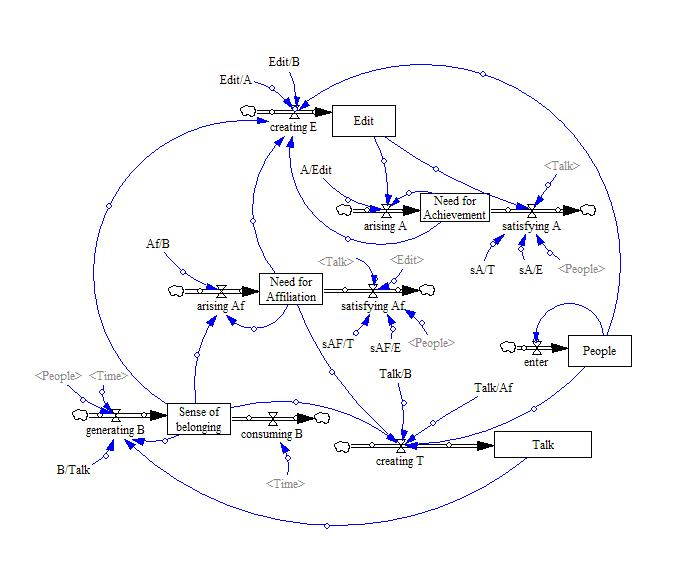
\includegraphics{05}}
    \caption{Data model }
  \end{figure}



\textrm{In the database design, the core table is
}\textrm{\textit{DRIVENRULES}}\textrm{. Complicated rules can be
decomposed into several Meta-rules that cannot be decomposed, and all
the rules are stored in }\textrm{\textit{DRIVENRULES}}\textrm{. Take
rule }\textrm{\textit{DR[2]}}\textrm{ and
}\textrm{\textit{DR[4]}}\textrm{ as example,
}\textrm{\textit{DR[4]}}\textrm{ itself is the Meta-rule, while three
Meta-rules would be generated after the decomposition of
}\textrm{\textit{DR[2]}}\textrm{, and according to the characters of
SMA, the relationship between the three generated rules is And.
Each rule will be executed in traverse until the last one. The store
result is depicted in Table 4.}

\begin{center}
\tablehead{}
\tablecaption{Example of driven rules}

\begin{supertabular}{m{0.6in}|m{0.95in}|m{0.88in}|m{0.88in}|m{0.88in}}
\hline
\centering \itshape\color{black} RuleID &
\centering \itshape\color{black}
RulePrecondition &
\centering \itshape\color{black} RuleConlusion &
\centering \itshape\color{black} RuleCategory &
\centering\arraybslash \itshape\color{black}
Super RuleID\\\hline
\centering \itshape\color{black} DR[2] &
\centering \sffamily
\textrm{\textit{\textcolor{black}{B}}}\textrm{\textit{\textcolor{black}{\textsuperscript{\^{}}}}}
&
\centering \itshape\color{black} KBM &
\centering \itshape\color{black} SMA &
~
\\
\centering \itshape\color{black} DR[20] &
\centering \sffamily
\textrm{\textit{\textcolor{black}{B}}}\textrm{\textit{\textcolor{black}{\textsuperscript{\^{}}}}}
&
\centering \itshape\color{black} KBCM &
\centering \itshape\color{black} SS &
\centering\arraybslash \itshape\color{black}
DR[2]\\
\centering \itshape\color{black} DR[21] &
\centering \sffamily
\textrm{\textit{\textcolor{black}{B}}}\textrm{\textit{\textcolor{black}{\textsuperscript{\^{}}}}}
&
\centering \itshape\color{black} SPM &
\centering \itshape\color{black} SS &
\centering\arraybslash \itshape\color{black}
DR[2]\\
\centering \itshape\color{black} DR[22] &
\centering \sffamily
\textrm{\textit{\textcolor{black}{B}}}\textrm{\textit{\textcolor{black}{\textsuperscript{\^{}}}}}
&
\centering \itshape\color{black} KBCP &
\centering \itshape\color{black} SS &
\centering\arraybslash \itshape\color{black}
DR[2]\\
\centering \itshape\color{black} DR[4] &
\centering \itshape\color{black} State+ &
\centering \itshape\color{black} KLA &
\centering \itshape\color{black} SS &
~
\\\hline
\end{supertabular}
\end{center}

\textrm{Meta-rules can be executed directly by the system; however real
driven-rules' execution  illustrated are mapped by
}\textrm{\textit{RulePrecondition}}\textrm{ and
}\textrm{\textit{RuleConclusion}}\textrm{, which represents one or one
group of indivisible actions. As a result, in database design, table
}\textrm{\textit{Expression}}\textrm{ is used to store the mapped
content from }\textrm{\textit{RulePrecondition}}\textrm{ and
}\textrm{\textit{RuleConclusion}}. \textrm{The primary key of
}\textrm{\textit{EXPRESSION}}\textrm{ is
}\textrm{\textit{ExpressionID}}\textrm{, representing the primary
indivisible actions. }\textrm{\textit{SuperExpressionID
}}\textrm{represents the entity that
}\textrm{\textit{ExpressionID}}\textrm{ belongs to, and the
}\textrm{\textit{ExpressionID}}\textrm{ is the most simple expressivity
if }\textrm{\textit{SuperExpressionID }}\textrm{is null. Take the
example of }\textrm{\textit{DR[2]}}\textrm{ and }\textrm{\textit{DR[4]
}}\textrm{again, the store result of all the expressivities is depicted
in Table 5.}

\begin{table}[!htb]
\tablehead{}
\tablecaption{ Example of expression}
\begin{supertabular}{m{2.13096in}|m{2.13096in}}
\hline
\centering \itshape\color{black} ExpressionID &
\centering\arraybslash \itshape\color{black}
SuperExpressionID\\\hline
\centering \sffamily
\textrm{\textit{\textcolor{black}{B}}}\textrm{\textit{\textcolor{black}{\textsuperscript{\^{}}}}}
&
~
\\
\centering \itshape\color{black} KBCM &
\centering\arraybslash \itshape\color{black}
KBM\\
\centering \itshape\color{black} SPM &
\centering\arraybslash \itshape\color{black}
KBM\\
\centering \itshape\color{black} KBCP &
\centering\arraybslash \itshape\color{black}
KBM\\
\centering \itshape\color{black} State+ &
~
\\
\centering \itshape\color{black} KLA &
~
\\\hline
\end{supertabular}
\end{table}

\textrm{The required parameters of each action also depend on the
parameters owned by these sub-}\textrm{expressivities.
Take}\textrm{\textit{ DR[2] }}\textrm{and DR[4] as example, the
executed expressivities and parameters are illustrated in Table 6 as
follows.}

\begin{table}[!htb]
\tablehead{}
\scriptsize{}
\tablecaption{Example of KBCM}
\begin{supertabular}{m{0.5in}|m{0.78in}|m{1.3in}|m{0.7in}|m{0.8in}}
\hline
\centering \bfseries\itshape\color{black} KBCMID
&
\centering \itshape\color{black} ExpressionID &
\centering \itshape\color{black} KBURI &
\centering \itshape\color{black} CN &
\centering\arraybslash \itshape\color{black}
NewCN\\\hline
\centering \itshape\color{black} 1 &
\centering \itshape\color{black} KBCM &
\centering \itshape\color{black}
urn:kbs:material/zgpx &
\centering \itshape\color{black}
zhigongpeixun &
\centering\arraybslash \itshape\color{black}
yuangongpeixun\\
\centering \itshape\color{black} 2 &
\centering \itshape\color{black} KBCM &
\centering \itshape\color{black}
urn:kbs:material/ck &
\centering \itshape\color{black} ciku
&
\centering\arraybslash \itshape\color{black}
zhuanyeciku\\
\centering \itshape\color{black} 3 &
\centering \itshape\color{black} KBCM &
\itshape\color{black} urn:kbs:material/zgpx/jcpx
&
\centering \itshape\color{black}
jichupeixun &
\centering\arraybslash \itshape\color{black}
jichupeixun\\\hline
\end{supertabular}
\end{table}


\textrm{From the example in Section 5, we know that KBCM is the action
that modify the knowledge base name, i.e.
}\textrm{\textit{KBCM}}\textrm{(}\textrm{\textit{URI,{\textless}CN,
CN'{\textgreater}}}\textrm{)}\textrm{\textit{,CN'${\neq}$0,
}}\textrm{where }\textrm{\textit{{\textless}CN,
CN'{\textgreater}}}\textrm{ represents modifying the knowledge base
name from }\textrm{\textit{CN}}\textrm{ to
}\textrm{\textit{CN'}}\textrm{, and
}\textrm{\textit{CN}}\textrm{' cannot be left empty.}


\textrm{If }\textrm{\textit{\textcolor{black}{CN= CN'}}}\textrm{, it
means that there's no change. In
}\textrm{\textit{KBCM}}\textrm{, column
}\textrm{\textit{KURUI}}\textrm{ corresponds to
}\textrm{\textit{URI}}\textrm{, column }\textrm{\textit{CN
}}\textrm{corresponds to}\textrm{\textit{ CN}}\textrm{, and
}\textrm{\textit{NewCN}}\textrm{ corresponds to
}\textrm{\textit{CN}}\textrm{'. An example
of}\textrm{\textit{ KBCM}}\textrm{ is displayed in Table 6.}


\textrm{\textit{KBCP}}\textrm{ refers to the action of modifying common
property in the knowledge base, i.e.
}\textrm{\textit{\textcolor{black}{KBCP}}}\textrm{\textcolor{black}{(}}\textrm{\textit{\textcolor{black}{{\textless}CP1,CP1'
{\textgreater};{\textless}CP2, CP2'
{\textgreater};…{\textless}CPn, CPn'
{\textgreater}}}}\textrm{\textcolor{black}{)}}\textrm{. In the ordered
pair
}\textrm{\textit{\textcolor{black}{{\textless}CPi,CPi'}}}\textit{\textcolor{black}{{\textgreater}}}\textrm{
, if }\textrm{\textit{\textcolor{black}{CPi' }}}\textrm{is null, it
means deleting; if }\textrm{\textit{\textcolor{black}{CPi}}}\textrm{ is
null while }\textrm{\textit{\textcolor{black}{CPi' }}}\textrm{is not
null, it means adding the property; and if
}\textrm{\textit{\textcolor{black}{CPi}}}\textrm{=}\textrm{\textit{\textcolor{black}{
CPi'}}}\textrm{\textcolor{black}{,}}\textrm{ it means
there's no change; if
}\textrm{\textit{\textcolor{black}{CPi'${\neq}$CPi}}}\textrm{, it means
to modify the common property from
}\textrm{\textit{\textcolor{black}{CPi}}}\textrm{ to
}\textrm{\textit{\textcolor{black}{CPi'}}}\textrm{\textcolor{black}{.
}}\textrm{In }\textrm{\textit{KBCP}}\textrm{, column
}\textrm{\textit{CP }}\textrm{corresponds to}\textrm{\textit{
CP}}\textrm{, and }\textrm{\textit{NewCP }}\textrm{corresponds to
}\textrm{\textit{CP}}\textrm{'. The storage of KBCP is
illustrated in Table 7.}

\begin{center}
\tablehead{}
\tablecaption{Example of KBCP}
\begin{supertabular}{m{0.7in}|m{1.1in}|m{1.1in}|m{1.1in}}
\hline
\centering \bfseries\itshape\color{black} KBCPID
&
\centering \itshape\color{black} ExpressionID &
\centering \itshape\color{black} CP &
\centering\arraybslash \itshape\color{black}
NewCP\\\hline
\centering \itshape\color{black} 1 &
\centering \itshape\color{black} KBCP &
\centering \itshape\color{black} Titile &
\centering\arraybslash \itshape\color{black}
Subject\\
\centering \itshape\color{black} 2 &
\centering \itshape\color{black} KBCP &
\centering \itshape\color{black} Summary &
\centering\arraybslash \itshape\color{black}
Abstract\\
\centering \itshape\color{black} 3 &
\centering \itshape\color{black} KBCP &
\centering \itshape\color{black} Author &
\centering\arraybslash \itshape\color{black}
Author\\
\centering \itshape\color{black} 4 &
\centering \itshape\color{black} KBCP &
~
 &
\centering\arraybslash \itshape\color{black}
SecurityLevel\\
\centering \itshape\color{black} 4 &
\centering \itshape\color{black} KBCP &
\centering \itshape\color{black} Location &
~
\\\hline
\end{supertabular}
\end{center}

\textrm{SPM refers to the action of modifying special property in the
knowledge base, i.e.
}\textrm{\textit{\textcolor{black}{SPM}}}\textrm{\textcolor{black}{(}}\textrm{\textit{\textcolor{black}{URI,
{\textless}SP1,SP1' {\textgreater};{\textless}SP2, SP2'
{\textgreater};…{\textless}SPn, SPn'
{\textgreater}}}}\textrm{\textcolor{black}{)}}\textrm{; where
}\textrm{\textit{URI}}\textrm{ represents the associated knowledge
base. In the ordered pair
}\textrm{\textit{\textcolor{black}{{\textless}SPi,SPi'}}}\textit{\textcolor{black}{{\textgreater}}}\textrm{
, if }\textrm{\textit{\textcolor{black}{SPi' }}}\textrm{is null, it
means deleting; if }\textrm{\textit{\textcolor{black}{SPi}}}\textrm{ is
null while }\textrm{\textit{\textcolor{black}{SPi' }}}\textrm{is not
null, it means adding the special property
}\textrm{\textit{\textcolor{black}{SPi' }}}\textrm{; and if
}\textrm{\textit{\textcolor{black}{SPi}}}\textrm{=}\textrm{\textit{\textcolor{black}{SPi'}}}\textrm{\textcolor{black}{,}}\textrm{
it means there's no change; if
}\textrm{\textit{\textcolor{black}{SPi'${\neq}$CPi}}}\textrm{, it means
to modify the common property from
}\textrm{\textit{\textcolor{black}{SPi}}}\textrm{ to
}\textrm{\textit{\textcolor{black}{SPi'}}}\textrm{\textcolor{black}{.
}}\textrm{In }\textrm{\textit{SPM}}\textrm{, column
}\textrm{\textit{KBRUI}}\textrm{ corresponds to
}\textrm{\textit{URI}}\textrm{, column }\textrm{\textit{SP
}}\textrm{corresponds to}\textrm{\textit{ SP}}\textrm{, and
}\textrm{\textit{NewSP }}\textrm{corresponds to
}\textrm{\textit{SP}}\textrm{'. The storage of
}\textrm{\textit{SPM}}\textrm{ is illustrated in Table 8.}

\begin{table}[!htb]
\tablehead{}
\tablecaption{Example of SPM}
\begin{supertabular}{m{0.45in}|m{0.8in}|m{1.31in}|m{0.78in}|m{0.7in}}
\hline
\centering \itshape\color{black} SPMID &
\centering \itshape\color{black} ExpressionID &
\centering \itshape\color{black} KBURI &
\centering \itshape\color{black} SP &
\centering\arraybslash \itshape\color{black}
NewSP\\\hline
\centering \itshape\color{black} 1 &
\centering \itshape\color{black} SPM &
\centering \itshape\color{black}
urn:kbs:material/gysxx &
\centering \itshape\color{black} Downloader &
\centering\arraybslash \itshape\color{black}
Reviewer\\
\centering \itshape\color{black} 2 &
\centering \itshape\color{black} SPM &
\centering \itshape\color{black}
urn:kbs:material/gysxx &
\centering \itshape\color{black} SellerName &
\centering\arraybslash \itshape\color{black}
Supplier\\
\centering \itshape\color{black} 3 &
\centering \itshape\color{black} SPM &
\centering \itshape\color{black}
urn:kbs:material/gysxx &
\centering \itshape\color{black} Version &
\centering\arraybslash \itshape\color{black}
Version\\
\centering \itshape\color{black} 4 &
\centering \itshape\color{black} SPM &
\centering \itshape\color{black}
urn:kbs:material/gysxx &
~
 &
\centering\arraybslash \itshape\color{black}
Code\\
\centering \itshape\color{black} 5 &
\centering \itshape\color{black} SPM &
\centering \itshape\color{black}
urn:kbs:material/gysxx &
\centering \itshape\color{black} IsUsing &
~
\\\hline
\end{supertabular}
\end{table}

\textrm{\textit{KLA}}\textrm{ is the action of adding knowledge state,
i.e.
}\textrm{\textit{\textcolor{black}{KLA}}}\textrm{\textcolor{black}{(}}\textrm{\textit{\textcolor{black}{KL\{LURI,LNA\}}}}\textrm{\textcolor{black}{),
where
}}$LURI$ \textrm{\textcolor{black}{
 represents the identification of the added knowledge state,
}}$LNA$
  represents the added knowledge state name. The storage example of
$KLA$  is
illustrated in Table 9 as follows:

\begin{center}
\tablehead{}
\tablecaption{Example of KLA}
\begin{supertabular}{m{0.4in}|m{0.8in}|m{1.78in}|m{0.8in}}
\hline
\centering \itshape\color{black} KLAID &
\centering \itshape\color{black} ExpressionID &
\centering \itshape\color{black} LURI &
\centering\arraybslash \itshape\color{black}
LNA\\\hline
\centering \itshape\color{black} 1 &
\centering \itshape\color{black} KLA &
\centering \sffamily
\textrm{\textit{\textcolor{black}{urn:kbs:lifestate/accreditating}}} &
\centering\arraybslash \itshape\color{black}
shending\\\hline
\end{supertabular}
\end{center}

\section{A Case
Study}
\label{sec:case-study-1}

\subsection{Application of the BP driven KMP modeling methodology}
\label{sec:appl-bp-driv-1}
\textrm{In order to understand the BP driven KMP modeling methodology
better, we use the case of the aviation manufacturing enterprise as
background to describe the application of the methodology. The BP model
of the enterprise has been depicted in Section 4. Assume that the
enterprise emphasize more on the reliability in its product design,
then each section in the design process would be under more strict
control. A new segment, Accrediting, should be added to the
original design process. The approved design proposal audited by
the directors cannot go into effect immediately. Instead, the proposal
has to be accredited by the institute leader. Only if it is
accredited by the institute leader can the proposal take effect
formally, otherwise it must be returned to the designer to be
modified. Therefore the state of "submit for
accrediting" has to be added in the state diagram, 
the section of "accredit design proposal"
should be added in the activity diagram, and the use case
"accredit the design proposal" is added for
the institute leader in the use case diagram.}


\textrm{The BP model of the product design for the enterprise is stored
in the global database. In the database design, we
view all the components in the state diagram as elements , which are
divided into five categories: state, action, judge, start and end. Each
element owns its }\textrm{\textit{ElementID}}\textrm{,
}\textrm{\textit{ElementName}}\textrm{,
}\textrm{\textit{PreElement}}\textrm{,
}\textrm{\textit{PastElement}}\textrm{ and
}\textrm{\textit{Flag,}}\textrm{ of which}\textrm{\textit{
ElementID}}\textrm{ is the primary key. The table structure is
illustrated in Table 10.}

\begin{table}[!ht]
\tablehead{}
\tablecaption{ Example of the storage of the state diagram}
\begin{supertabular}{m{0.6in}m{1.1052598in}m{1.1in}m{1in}m{0.4in}}
\hline
\bfseries\itshape ElementID &
 \bfseries\itshape PreElement &
 \bfseries\itshape ElementName &
 \bfseries\itshape PostElement &
\arraybslash \bfseries\itshape
Flag\\\hline
\centering \itshape 1 &
\itshape Null &
\itshape Starting &
\itshape InputSave &
\itshape Start\\
\centering \itshape 2 &
\itshape Starting &
\itshape InputSave &
\itshape Draft &
\itshape Action\\
\centering \itshape 3 &
\itshape InputSave &
\itshape Draft &
\itshape Submit &
\itshape State\\
\centering \itshape 4 &
\itshape Draft &
\itshape Submit &
\itshape Examining &
\itshape Action\\
\centering \itshape 5 &
\itshape Submit &
\itshape Examining &
\itshape Examine &
\itshape State\\
\centering \itshape 6 &
\itshape Examining &
\itshape Examine &
\itshape PassExamine &
\itshape Action\\
\centering \itshape 7 &
\itshape Examining &
\itshape Examine &
\itshape FailExamine &
\itshape Action\\
\centering \itshape 8 &
\itshape Examine &
\itshape PassExamine &
\itshape Censoring &
\itshape Judge\\
\centering \itshape 9 &
\itshape Examine &
\itshape FailExamine &
\itshape FailExamineState &
\itshape Judge\\
\centering \itshape 10 &
\itshape PassExamine &
\itshape Censoring &
\itshape Censor &
\itshape State\\
\centering \itshape 11 &
\itshape FailExamine &
\itshape FailExamineState &
\itshape FailExValueCheck &
\itshape State\\
\centering \itshape 12 &
\itshape FailExamineState &
\itshape FailExValueCheck &
\itshape Valuable &
\itshape Action\\
\centering \itshape 13 &
\itshape FailExamineState &
\itshape FailExValueCheck &
\itshape Valueless &
\itshape Action\\
\centering \itshape 14 &
\itshape\color{black} FailExValueCheck &
\itshape\color{black} Valuable &
\itshape\color{black} Draft &
\itshape\color{black} Judge\\
\centering \itshape 15 &
\itshape\color{black} FailCenValueCheck &
\itshape\color{black} Valuable &
\itshape\color{black} Draft &
\itshape\color{black} Judge\\
\centering \itshape 16 &
\itshape\color{black} FailExValueCheck &
\itshape\color{black} Valueless &
\itshape\color{black} Eliminated &
\itshape\color{black} Judge\\
\centering \itshape 17 &
\itshape\color{black} FailCenValueCheck &
\itshape\color{black} Valueless &
\itshape\color{black} Eliminated &
\itshape\color{black} Judge\\
\centering \itshape 18 &
\itshape Censoring &
\itshape Censor &
\itshape PassCensor &
\itshape Action\\
\centering \itshape 19 &
\itshape Censoring &
\itshape Censor &
\itshape FailCensor &
\itshape Action\\
\centering \itshape 20 &
\itshape Censor &
\itshape PassCensor &
\itshape Published &
\itshape Judge\\
\centering \itshape 21 &
\itshape Censor &
\itshape FailCensor &
\itshape FailCensorState &
\itshape Judge\\
\centering \itshape 22 &
\itshape PassCensor &
\itshape Published &
\itshape End &
\itshape State\\
\centering \itshape 23 &
\itshape FailCensor &
\itshape FailCensorState &
\itshape FailCenValueCheck &
\itshape State\\
\centering \itshape 24 &
\itshape FailCensorState &
\itshape FailCenValueCheck &
\itshape Valuable &
\itshape Action\\
\centering \itshape 25 &
\itshape FailCensorState &
\itshape FailCenValueCheck &
\itshape Valueless &
\itshape Action\\
\centering \itshape 26 &
\itshape Valueless &
\itshape Eliminated &
\itshape Ending &
\itshape State\\
\centering \itshape 27 &
\itshape Published &
\itshape Ending &
\sffamily
\textrm{\textit{Null}}\textrm{\textcolor{black}{ }} &
\itshape End\\
\centering \itshape 28 &
\itshape Eliminated &
\itshape Ending &
\itshape Null &
\itshape End\\\hline
\end{supertabular}
\end{table}


 All the BP models can split the elements and
store them in such tables. Through the stored
elements in the table, the specific BP models can also be recovered. The
store result of the state diagram in the case (Fig.2) is displayed in
Table 10. The new BP model is shown in Fig.6.



  \begin{figure}[!t]
    \centering
    \scalebox{0.7}{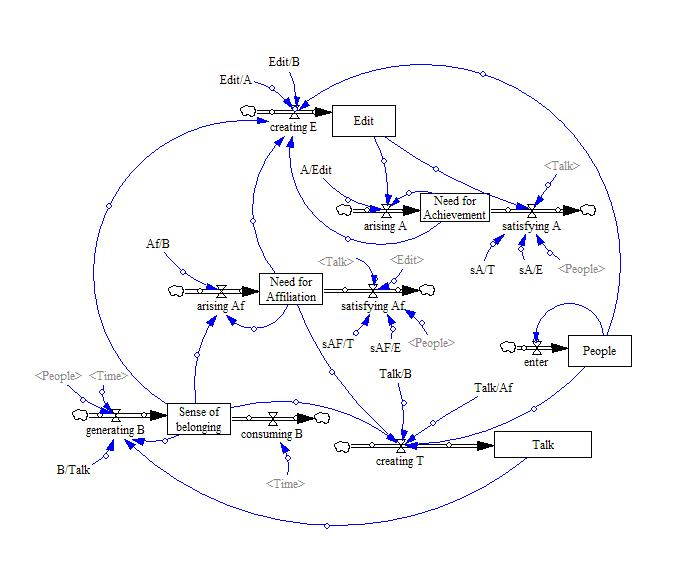
\includegraphics{06}}
    \caption{ The state diagram in which the state of Accrediting has been added }
  \end{figure}

\textrm{After users' inputting new BP model, some
elements in the original table will be changed. In Table 8, the
elements with the }\textrm{\textit{ElementID}}\textrm{
"20" and "22"
would be changed. The }\textrm{\textit{PostElement}}\textrm{ of
"}\textrm{\textit{PassCensor}}\textrm{"
with }\textrm{\textit{ElementID}}\textrm{
"20" should be changed to
"}\textrm{\textit{Accrediting}}\textrm{";
therefore, when
"}\textrm{\textit{PassCensor}}\textrm{" is
the }\textrm{\textit{PreElement}}\textrm{, the current element is
"}\textrm{\textit{Accrediting}}\textrm{"
with "}\textrm{\textit{Accredit}}\textrm{"
as its }\textrm{\textit{PostElement}}\textrm{. Moreover, elements with
}\textrm{\textit{ElementID}}\textrm{
"29-38" are the new added elements. Part of
the store results of the new BP models in the database are displayed in
Table 11 (Only the changes are stored).}

\begin{table}[!b]
\tablehead{}
\tablecaption{ Example of the new state diagram storage (the changed part)}
\begin{supertabular}{m{0.6in}m{1.1052598in}m{1.1in}m{1in}m{0.4in}}
\hline
\bfseries\itshape ElementID &
\bfseries\itshape PreElement &
\bfseries\itshape ElementName &
\bfseries\itshape PostElement &
\bfseries\itshape Flag\\\hline
\itshape 29 &
\itshape FailAccValueCheck &
\itshape Valuable &
\itshape Draft &
\itshape Judge\\
\itshape 30 &
\itshape FailAccValueCheck &
\itshape Valueless &
\itshape Elimated &
\itshape Judge\\
\itshape 20 &
\itshape Censor &
\itshape PassCensor &
\itshape Accrediting &
\itshape Judge\\
\itshape 22 &
\itshape PassCensor &
\itshape Accrediting &
\itshape Accredit &
\itshape State\\
\itshape 31 &
\itshape Accrediting &
\itshape Accredit &
\itshape PassAccredit &
\itshape Action\\
\itshape 32 &
\itshape Accrediting &
\itshape Accredit &
\itshape FailAccredit &
\itshape Action\\
\itshape 33 &
\itshape Accredit &
\itshape PassAccredit &
\itshape Published &
\itshape Judge\\
\itshape 34 &
\itshape Accredit &
\itshape FailAccredit &
\itshape FailAccreditState &
\itshape Judge\\
\itshape 35 &
\itshape PassAccredit &
\itshape Published &
\itshape Ending &
\itshape State\\
\itshape 36 &
\itshape Fail Accredit &
\itshape Fail AccreditState &
\itshape FailAccValueCheck &
\itshape State\\
\itshape 37 &
\itshape FailAccreditState &
\itshape FailAccValueCheck &
\itshape Valuable &
\itshape Action\\
\itshape 38 &
\itshape FailAccreditState &
\itshape FailAccValueCheck &
\itshape Valueless &
\itshape Action\\\hline
\end{supertabular}
\end{table}

\textrm{The prototype functions of }\textrm{\textit{BDKMS}}\textrm{
mainly includes: BP input, BP driven KMP modeling and driven-rules
maintenance, etc. Its user interface is depicted in Fig.7.}

  \begin{figure}[ht]
    \centering
    \scalebox{0.62}{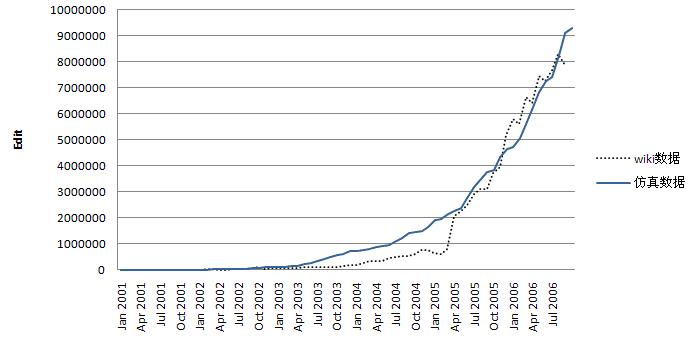
\includegraphics{07}}
    \caption{  The prototype of BDKMS}
  \end{figure}


\textrm{User input the new BP model into the
}\textrm{\textit{BDKMS}}\textrm{, in which a new section of
"Accrediting" is added, and then the system
would compare it with the original BP model to resolve the changes of
the BP; finally the Driver is triggered to work. The Driver will search
corresponding rules in the driven-rules base according to the changed
parameters. In the case, the rule is }$DR[4]=IF \ State^+
\ THEN \ KLA$\textrm{, where
}\textrm{\textit{KLA=KLA}}\textrm{(}\textrm{\textit{KL\{LURI,LNA\}}}\textrm{).
The Inference Engine would implement inference according to the
inference principles in Section 6.2, and generate the required
parameters of the KMP modeling (i.e. state identification
}\textrm{\textit{LURI=}}\textrm{\textbf{\textit{
}}}\textrm{\textit{urn:kbs:lifestate/accredit}}\textrm{, state name
}\textrm{\textit{LNA=“accrediting”}}) according to the standard
of the Knowledge State ({KL), then the
parameter is input into the KMP model in the global database to drive
the model change. Then the new KMP model would be explained by
the Explanatory and presented to the users through the User Interface
as well. The added state in KMP moedel is illustrated in Fig.8.


  \begin{figure}[ht]
    \centering
    \scalebox{0.75}{\includegraphics{08}}
    \caption{ The graph of the new KMP model}
  \end{figure}



In the new KMP model documents generated by the system, the section of
"Accrediting" is also added to the KMP. The
segment of corresponding XML documents is as follows:

{\itshape
{\textless}kid:id rdf:about="urn:kbs:lifestate/
accreditating "{\textgreater}}

{\itshape
\ \ {\textless}kid:is
rdf:resource="urn:kbs:lifestate"
/{\textgreater}}

{\itshape
{\textless}/kid:id{\textgreater}}

{
The KMS could reflect the new KMP in the system by the new XML
documents. In this case, the section of Accrediting by the institute
leader is added in the process of knowledge publishing; similarly, the
section of Accrediting is added to knowledge downloading, modifying and
pigeonholing.}

\subsection{ Evaluation of the method application}
\label{sec:eval-meth-appl-1}

The method of BP Driven KMP Modeling
(BDKM) has been applied for test in the
aviation manufacturing enterprise. In order to evaluate the method
, this paper compare some critical factors before and after
implementing the system, as is illustrated in Table 12. These data were
collected and summarized by the enterprise. Each period lasts 6 months. 
\begin{table}[hbt]
\tablehead{}
\tablecaption{Evaluation of  BDKMS
application in the aviation manufacturing enterprise}
\scriptsize{}
\begin{supertabular}{m{0.7in}|m{0.9in}|m{1.2in}|m{0.6in}|m{0.6in}|m{0.66in}}
\hline
\centering \bfseries classification &
\centering \bfseries Evaluation Factors &
\centering \sffamily \textrm{\textbf{Measurement
Units}} &
\centering \sffamily \textrm{\textbf{The results
before }}\textrm{\textbf{\textit{BDKM}}} &
\centering \sffamily \textrm{\textbf{The results
after }}\textrm{\textbf{\textit{BDKM}}} &
\centering\arraybslash \bfseries Improved
Degree\\\hline
\sffamily \textrm{T}\textrm{he perspective of
KMP} &
\sffamily \textrm{Accuracy} &
\sffamily \textrm{Error rate/The time to
maintain a single node} &
 70\%-80\% &
 10\%-20\% &
 71.4\%-87.5\%\\
 &
 Efficiency &
\sffamily \textrm{/The number of people involved
in maintaining a single business node} &
 3h-8h &
 0.3h-1h &
 66.7\%-96.3\%\\
 &
 Number of maintenance staff &
~
 &
\sffamily \textrm{4-6 people} &
\sffamily \textrm{1-2 people} &
 50\%-83.3\%\\
 &
 Staff Cost &
\sffamily \textrm{Cost/Maintaining team} &
 \$100-\$150 &
 \$20-\$30 &
 70\%-86\%\\
 &
 Dependency on experts &
\sffamily \textrm{Experts engaging time/Maintain
a single business node} &
 2.5h-7h &
 0.1h-0.5h &
 80\%-98.6\%\\\hline
 The perspective of customer service &
 Demand Response &
\sffamily \textrm{Responsive time/single
requirement} &
\sffamily \textrm{About 4.5 days} &
\sffamily \textrm{About 1.5days} &
 66.7\%\\
 &
 Customer Satisfactory &
\sffamily \textrm{The average degree of
satisfaction(full marks: 7 points)/month} &
 4.3 &
 6.8 &
 58.1\%\\\hline
 The perspective of management &
 Responsive Efficiency to the BP change &
\sffamily \textrm{Decision time/Business change}
&
 2-8h &
 0.1-0.3h &
 85\%-99\%\\
 &
 Responsive effect of the KM to business change
&
\sffamily \textrm{The average degree of
satisfaction in response(full marks: 10 points)/Business change} &
\sffamily \textrm{6.4} &
 8.7 &
 35.9\%\\\hline
\end{supertabular}
\end{table}

We also make a
radar chart according to the data in Table 12 to display the
improvement after BDKMS application. As shown in Fig.9, each
evaluation factor is rescaled by logarithmic transformation to make
the chart more clearly. At the same time, the dimensions of customer
satisfactory and responsive effect are both preprocessed to meet the
whole improving trend.
\begin{figure}[!hb]
  \centering
  \scalebox{0.35}{\includegraphics{09}}
  \caption{The Radar Chart of the BDKMS application evaluation}
\end{figure}
 We can know
from table 12 that the methodology of \textrm{\textit{BDKM}}\textrm{
greatly optimizes the maintenance of enterprises' KMP.
The accuracy increased and time has been
reduced by more than 60\%. The dependency on experts has greatly
decreased, and the improvement in this aspect is enormously outstanding
with an 80\% improved degree. Besides, the
improvement of KMP maintenance also influences customer service. It is
mainly embodied in the fact that the corresponding time has been
reduced by 67\%, and customer satisfaction has increased by more than
50\%. Moreover, the BP driven factors also improve the management
efficiency from the perspective of management, mainly the BP change
management. After the BP change, the management team has to act to the
change as soon as possible to set down the strategies of KM change.
With the method of }\textrm{\textit{BDKM}}\textrm{, some manual
decisions has been substituted by driven-rules in the method. Therefore
the decision efficiency has increased by over 80\%, and the effects on
decision-making has also risen by more than 30\%.}


In conclusion, all the results in the application illustrate that the
method of BDKPM has great superiority, which largely promote the
optimization of KMP, and in turn promote the optimization of BP; as a
result the whole benefit and competiveness of the enterprise is
improved.

\section{Conclusion}
\label{sec:conclusion-1}

\textrm{Knowledge Management Process (KMP) is a continually improved
process, and it is the close relationship with Business Process (BP)
that drives continual improvement. On the basis of this thought, we
propose a BP driven KMP modeling method in this paper. This method
includes the architecture of BP driven KMP modeling system, depiction
of BP model, method of KMP modeling, description of the driven-rules
between BP and KMP as well as its storage, etc. In the end, this paper
uses the designing institute of an aviation manufacturing enterprise as
background to depict the application of the method, and evaluate the
method finally. The results show that this method can promote the
collaboration between BP and KMP effectively, and realize BP driven
automation to some extent to promote the optimization and continual
improvement. Nevertheless, there still exist some shortcomings in this
paper. For example, the prototype case is incomplete, and the
automation of BP driven is not sufficient, which requires further
research in the future.}


\bibliographystyle{elsarticle-harv}
% \bibliography{bib2}
\begin{thebibliography}{37}
\expandafter\ifx\csname natexlab\endcsname\relax\def\natexlab#1{#1}\fi
\expandafter\ifx\csname url\endcsname\relax
  \def\url#1{\texttt{#1}}\fi
\expandafter\ifx\csname urlprefix\endcsname\relax\def\urlprefix{URL }\fi

\bibitem[{Ahn et~al.(2005)Ahn, Lee, Cho, and Park}]{ahn2005utilizing}
Ahn, H., Lee, H., Cho, K., Park, S., 2005. {Utilizing knowledge context in
  virtual collaborative work}. Decision Support Systems 39~(4), 563--582.

\bibitem[{Alavi and Leidner(2001)}]{alavi2001review}
Alavi, M., Leidner, D., 2001. {Review: Knowledge management and knowledge
  management systems: Conceptual foundations and research issues}. MIS
  quarterly, 107--136.

\bibitem[{Ballard et~al.(2005)Ballard, White, McDonald, Mylymaki, McDowell,
  Goerlich, and Neroda}]{ballard2005business}
Ballard, C., White, C., McDonald, S., Mylymaki, J., McDowell, S., Goerlich, O.,
  Neroda, A., 2005. {Business performance management: meets business
  intelligence}. IBM.

\bibitem[{Becerra-Fernandez and Sabherwal(2001)}]{becerra2001organizational}
Becerra-Fernandez, I., Sabherwal, R., 2001. {Organizational knowledge
  management: A contingency perspective}. Journal of Management Information
  Systems 18~(1), 23--55.

\bibitem[{Berggren et~al.(1998)Berggren, Bjarnason, Johansson, and
  Walczak}]{berggren1998knowledge}
Berggren, C., Bjarnason, B., Johansson, G., Walczak, S., 1998. {Knowledge
  acquisition and knowledge representation with class: the object-oriented
  paradigm}. Expert Systems with Applications 15~(3), 235--244.

\bibitem[{Berztiss(2000)}]{berztiss2000knowledge}
Berztiss, A., 2000. {Knowledge and workflow systems}. In: Proceedings of the
  11th International Workshop on Database and Expert Systems Applications. IEEE
  Computer Society Washington, DC, USA, p. 1102.

\bibitem[{Chau and Albermani(2002)}]{chau2002expert}
Chau, K., Albermani, F., 2002. {Expert system application on preliminary design
  of water retaining structures}. Expert systems with applications 22~(2),
  169--178.

\bibitem[{Chen et~al.(2005)Chen, Chen, Wang, Chu, and
  Tsai}]{chen2005developing}
Chen, Y., Chen, Y., Wang, C., Chu, H., Tsai, T., 2005. {Developing a
  multi-layer reference design retrieval technology for knowledge management in
  engineering design}. Expert Systems with Applications 29~(4), 839--866.

\bibitem[{Choi et~al.(2004)Choi, Jung, and Song}]{choi2004integrated}
Choi, I., Jung, J., Song, M., 2004. {An integrated framework for process
  knowledge management}. International Journal of Innovation and Learning
  1~(4), 399--408.

\bibitem[{Chung et~al.(2003)Chung, Cheung, Stader, Jarvis, Moore, and
  Macintosh}]{chung2003knowledge}
Chung, P., Cheung, L., Stader, J., Jarvis, P., Moore, J., Macintosh, A., 2003.
  {Knowledge-based process management—an approach to handling adaptive
  workflow}. Knowledge-Based Systems 16~(3), 149--160.

\bibitem[{Curtis and Cobham(2005)}]{curtis2005business}
Curtis, G., Cobham, D., 2005. {Business information systems: analysis, design,
  and practice}. Pearson Education.

\bibitem[{Dalkir(2005)}]{dalkir2005knowledge}
Dalkir, K., 2005. {Knowledge management in theory and practice}.
  Butterworth-Heinemann.

\bibitem[{Davenport and Prusak(1998)}]{davenport1998working}
Davenport, T., Prusak, L., 1998. {Working knowledge: How organizations manage
  what they know}. Harvard Business School Pr.

\bibitem[{Desouza(2003)}]{desouza2003barriers}
Desouza, K., 2003. {Barriers to effective use of knowledge management systems
  in software engineering}. Communications of the ACM 46~(1), 99--101.

\bibitem[{Desouza et~al.(2006)Desouza, Awazu, and Tiwana}]{desouza2006four}
Desouza, K., Awazu, Y., Tiwana, A., 2006. {Four dynamics for bringing use back
  into software reuse}. Communications of the ACM 49~(1), 96--100.

\bibitem[{Dhaliwal and Benbasat(1996)}]{dhaliwal1996use}
Dhaliwal, J., Benbasat, I., 1996. {The use and effects of knowledge-based
  system explanations: theoretical foundations and a framework for empirical
  evaluation}. Information Systems Research 7~(3), 342.

\bibitem[{Hammer and Champy(2003)}]{hammer2003reengineering}
Hammer, M., Champy, J., 2003. {Reengineering the corporation: A manifesto for
  business revolution}. Collins Business.

\bibitem[{Han and Park(2009)}]{han2009process}
Han, K., Park, J., 2009. {Process-centered knowledge model and enterprise
  ontology for the development of knowledge management system}. Expert Systems
  with Applications 36~(4), 7441--7447.

\bibitem[{Huang(2009)}]{huang2009designing}
Huang, H., 2009. {Designing a knowledge-based system for strategic planning: A
  balanced scorecard perspective}. Expert Systems with Applications 36~(1),
  209--218.

\bibitem[{Jablonski et~al.(2001)Jablonski, Horn, and
  Schlundt}]{jablonski-process}
Jablonski, S., Horn, S., Schlundt, M., 2001. {Process oriented knowledge
  management}. In: Eleventh International Workshop on Research Issues in Data
  Engineering: Document Management for Data Intensive Business and Scientific
  Applications, Heidelberg, Germany. pp. 77--84.

\bibitem[{Jovanovic and Ga{\v{s}}evic(2005)}]{jovanovic2005achieving}
Jovanovic, J., Ga{\v{s}}evic, D., 2005. {Achieving knowledge interoperability:
  An XML/XSLT approach}. Expert Systems with Applications 29~(3), 535--553.

\bibitem[{Jung et~al.(2007)Jung, Choi, and Song}]{jung2007integration}
Jung, J., Choi, I., Song, M., 2007. {An integration architecture for knowledge
  management systems and business process management systems}. Computers in
  industry 58~(1), 21--34.

\bibitem[{Kang(2007)}]{kang2007process}
Kang, K., 2007. {A process-based performance measurement framework for
  continuous process improvement}. International Journal of Industrial
  Engineering 14~(3).

\bibitem[{Kueng and Kawalek(1997)}]{kueng1997goal}
Kueng, P., Kawalek, P., 1997. {Goal-based business process models: creation and
  evaluation}. Business Process Management Journal 3~(1), 17--38.

\bibitem[{Lai and Fan(2002)}]{lai2002workflow}
Lai, J., Fan, Y., 2002. {Workflow and knowledge management: approaching an
  integration}. Lecture Notes in Computer Science, 16--29.

\bibitem[{Macio{\l}(2008)}]{maciol2008application}
Macio{\l}, A., 2008. {An application of rule-based tool in attributive logic
  for business rules modeling}. Expert Systems with Applications 34~(3),
  1825--1836.

\bibitem[{Maurer and Dellen(1998)}]{maurer98concept}
Maurer, F., Dellen, B., 1998. {A concept for an internet-based process-oriented
  knowledge management environment}. In: Proceedings of the KAW. pp. 18--23.

\bibitem[{Maurer et~al.(2000)Maurer, Dellen, Bendeck, Goldmann, Holz, Kotting,
  and Schaaf}]{maurer2000merging}
Maurer, F., Dellen, B., Bendeck, F., Goldmann, S., Holz, H., Kotting, B.,
  Schaaf, M., 2000. {Merging project planning and Web enabled dynamic workflow
  technologies}. IEEE Internet Computing 4~(3), 65--74.

\bibitem[{Maurer and Holz(1999)}]{maurer1999process}
Maurer, F., Holz, H., 1999. {Process-oriented knowledge management for learning
  software organizations}. In: Proceedings of 12th Knowledge Acquisition For
  Knowledge-Based Systems Workshop. Citeseer.

\bibitem[{Millie~Kwan and Balasubramanian(2003)}]{millie2003knowledgescope}
Millie~Kwan, M., Balasubramanian, P., 2003. {KnowledgeScope: managing knowledge
  in context}. Decision Support Systems 35~(4), 467--486.

\bibitem[{Nissen et~al.(2000)Nissen, Kamel, and Sengupta}]{nissen2000toward}
Nissen, M., Kamel, M., Sengupta, K., 2000. {Toward integrating knowledge
  management, processes and systems: a position paper}. In: American
  Association for Artificial Intelligence 2000 Spring Symposium, Stanford, CA,
  Workshop on Bringing Knowledge to Business Processes (March 2000).

\bibitem[{Raghu and Vinze(2007)}]{raghu2007business}
Raghu, T., Vinze, A., 2007. {A business process context for Knowledge
  Management}. Decision Support Systems 43~(3), 1062--1079.

\bibitem[{Vandaie(2008)}]{vandaie2008role}
Vandaie, R., 2008. {The role of organizational knowledge management in
  successful ERP implementation projects}. Knowledge-Based Systems 21~(8),
  920--926.

\bibitem[{Wen et~al.(2008)Wen, Chen, and Pao}]{wen2008mobile}
Wen, W., Chen, Y., Pao, H., 2008. {A mobile knowledge management decision
  support system for automatically conducting an electronic business}.
  Knowledge-Based Systems 21~(7), 540--550.

\bibitem[{Woitsch and Karagiannis(2005)}]{woitsch2005process}
Woitsch, R., Karagiannis, D., 2005. {Process Oriented Knowledge Management: A
  Service Based Approach}. Journal of Universal Computer Science 11~(4),
  565--588.

\bibitem[{Yang et~al.(2009)Yang, Miao, Wu, and Zhou}]{yang2009product}
Yang, D., Miao, R., Wu, H., Zhou, Y., 2009. {Product configuration knowledge
  modeling using ontology web language}. Expert Systems with Applications
  36~(3P1), 4399--4411.

\bibitem[{Zhao et~al.(2006)Zhao, Bi, Chen, Zeng, Lin, and
  Chau}]{zhao2006process}
Zhao, J., Bi, H., Chen, H., Zeng, D., Lin, C., Chau, M., 2006. {Process-driven
  collaboration support for intra-agency crime analysis}. Decision Support
  Systems 41~(3), 616--633.

\end{thebibliography}

\end{document}